\chapter{Theory and Methods \label{chap: Methods}}

In this chapter we describe the two methods that we will use to compute the density of states in this project. Using the ballistic transport method, we will obtain an exact analytical expression of this quantity for non-interacting systems (\ref{sec:transport}). The physics of interacting systems is more complex and does not support an exact approach. Instead, we appeal to the renown numerical renormalization group (NRG) to deal with the strong correlations of these systems \ref{sec:The-Numerical-Renormaliztion} . Both models will be tested on the model of a double quantum dot attached to a metallic lead.
We will observe that at very low energies, the physics of interacting systems emulates characteristic features of non-interacting models. 


\section{Ballistic transport \label{sec:transport} }

The Green function $G$ of a Hamiltonian $H$ is the operator that satisfies the homogeneous equation 
\begin{equation}
    \left(i\hbar\frac{\partial}{\partial t}-H\right)G\left(t-t'\right)=\delta(t-t').
\end{equation}

This type of differential equations are solved taking the Fourier transform 
\begin{equation}
    \Green{H}=\int_{-\infty}^{\infty}G(t-t')e^{i\omega(t-t')/\hbar}\delta(t-t')
\end{equation}

In this new space the solution of the equation is 
$$(\omega+is -H)\Green{\omega}=I.$$ 

The term $+is$ in the previous Hamiltonian is part of a mathematical trick quite common in this theory. During the whole procedure, the Green function acts on the complex field. But when we need to obtain a physical interpretation we will take the limit $s\rightarrow0$ to obtain the result for real energies. 

The next step is to decompose $\Green{H}$ in the eigenbase of the Hamiltonian $\{\ket{\alpha}\}$  by 


\begin{equation}
    \langle \alpha  \vert \Green{H}\ket{\alpha'}=\frac{\delta_{\alpha\alpha'}}{\omega - is -\ep_\alpha}=\frac{\delta_{\alpha\alpha'}(\omega + is -\ep_\alpha)}{(\omega-\epsilon_{\alpha})^{2}+s^{2}}.
\end{equation}

From the famous formula 
\begin{equation}
\lim_{s\rightarrow0}\frac{s}{(\omega-\epsilon_{\alpha})^{2}+s^{2}}=\pi\delta(\omega-\epsilon_{\alpha})
\end{equation}
we obtain 
\begin{equation}
    Im \langle \alpha  \vert \Green{H}\ket{\alpha'}] = \pi \delta(\omega -\epsilon_\alpha)\delta_{\alpha,\alpha'}.
\end{equation}
Note that the sum of $Im[ \langle \alpha  \vert \Green{H}\ket{\alpha'}]$ over all the eigenstates of $H$ is simply $\pi$ times the density of states:

\begin{equation}
    \rho(\omega)=-\frac{1}{\pi} \sum_\alpha Im \left[ \langle \alpha  \vert \Green{H}\ket{\alpha'}\right] = \sum_\alpha \delta(\omega-\epsilon_\alpha) . \label{eq:DOS_def}
\end{equation}

An extended definition of the Green function  can be given in terms of fermion operators in second quantization.  The time-green function for two fermion operators $A$ and $B$ is
\begin{equation}
  G_{A,B}(t-t') = \mathbb{T}[\{ A(t),B(t') \} ]. \label{eq:TempGreen}
\end{equation}
In these problems, causality is important, which is the reason why we use the time-order operator $\mathbb{T}$.  In addition, the evolution of this Green function is determined by Schroedinger's differential equation. 
\begin{equation}
\frac{d}{dt}G_{A,B}\left(t-t'\right)=\langle\left[A(t),B(t')\right]\rangle\delta_{t-t'}+\langle\left[A(t),H'\right],B(t')\rangle
\label{eq:Motion}
\end{equation}

Once again, we perform a Fourier transform of $G_{A,B}(t-t') $ to obtain $\Green{A,B}$. When applying this transform to \ref{eq:Motion} we obtain 

\begin{equation}
    \omega\Green{A,B}=\delta_{A^{\dagger},B}+\Green{\left[A,H\right],B}.
    \label{eq:Transport}
\end{equation}


\noindent Applying \ref{eq:Transport}  to a set of operators $\{A_1, A_2, \ldots \}$ we obtain a whole set of transport equations describing the flow of state transitions of the operators in our model. In this thesis we will identify each set of equations with a flow graph. This will be our leading method to compute the green functions of the system.

Moreover, following equation \ref{eq:DOS_def} we can define the density of states associated to an operator $A$ as

\begin{equation}
    \rho_{A,A^\dagger}=-\frac{1}{\pi}Im\left[\Green{A,A^\dagger}\right].
    \label{eq:Density of States}
\end{equation}

\noindent The density of states contains important physical information related to operator $A$. In our case, operator $A^\dagger$ will be related to the dot's creation operator  $d^\dagger$. Hence computing \ref{eq:Density of States} will allow us to observe the hybridization of the dot's discrete states and the creation of other energy levels due to the interaction with the lead and other possible impurities. We will observe examples of these computations in the following sections.


% ----------------------------- Graph Method-----------------------
\subsection{Using Graph Theory to Solve Ballistic Transport Equations \label{sec:GraphMethod}}


Solving the transport equations involves dealing with a set of linear equations where all the possible variables including  $\omega$ , and the Hamiltonian parameters are assumed to be constant.  This can be done by  Gauss-Jordan elimination, noting that after each elimination process we need to carry on the account in terms of the initial  variables. The solution  will be a polynomial fraction.  When the number of operators in the Hamiltonian increases the number of terms in the polynomial grows-up rapidly according to the number of initial parameters. This reveals the importance of exploring new methods that could simplify the solution of this system, and present a readable factorized expression of the final solution.   \\

The method presented here uses graph theory algorithms that provide a shortcut to Gauss-Jordan elimination \cite{spielman10}. To probe this method we solve here the transport equations for a non-interacting $(U=0)$ DQD connected to one lead. 

According to the Anderson model the Hamiltonian for this system looks like 
\begin{equation}
    H=\sum_{i=1}^2\epsilon_{di}d_{i}^{\dagger}d_{i}+ t_{dots}d_{1}^{\dagger}d_{2}+t_{dots}^*d_{2}^{\dagger}d_{1}+\sum_{k}\left(V_{i}d_{i}^{\dagger}c_{\mathbf{k}}+V_{i}^{*}c_{\mathbf{k}}^{\dagger}d_{i}\right) + \epsilon_{\mathbf{k}}c_{\mathbf{k}}^{\dagger}c_{\mathbf{k}}.
    \label{eq:HDQD}
\end{equation} 
\noindent Since the system is non-interacting, we ignore the spin-degeneracy of this Hamiltonian. The only new parameter here is the term $t_{dots}$, which represents the tunneling between both quantum dots.  Using equation \eqref{eq:Transport} with $B = d_1^\dagger$ and $A$ shifting among other operators we compute the following  transport equations
\begin{align}
     \left(\omega-\epsilon_{1}\right)\Green{d_{1},d_{1}^{\dagger}}&=1+t_{dots}\Green{d_{2},d_{1}^{\dagger}}+V_{1}^{*}\sum_{\mathbf{k}}\Green{c_{\mathbf{k}},d_{1}^{\dagger}} \label{eq:green1}  \\
     \left(\omega-\epsilon_{\mathbf{k}}\right)\Green{c_{\mathbf{k}},d_{1}^{\dagger}} &= V_{1}\Green{d_{1},d_{1}^{\dagger}}+V_{2}\Green{d_{2},d_{1}^{\dagger}} \label{eq:green2} \\
     \left(\omega-\epsilon_{2}\right)\Green{d_{2},d_{1}^{\dagger}}&= t_{dots}\Green{d_{1},d_{1}^{\dagger}}+V_{2}^{*}\sum_{\mathbf{k}}\Green{c_{\mathbf{k}},d_{1}^{\dagger}} \label{eq:green3} 
\end{align}
    %  \left(\omega-\epsilon_{1}\right)\Green{d_{1},d_{1}^{\dagger}}	= & 1+t_{dots}\Green{d_{2},d_{1}^{\dagger}}+V_{1}^{*}\sum_{\mathbf{k}}\Green{c_{\mathbf{k}},d_{1}^{\dagger}} \\

    % \left(\omega-\epsilon_{\mathbf{k}}\right)\Green{c_{\mathbf{k}},d_{1}^{\dagger}}= & V_{1}\Green{d_{1},d_{1}^{\dagger}}+V_{2}\Green{d_{2},d_{1}^{\dagger}} \\

    % \left(\omega-\epsilon_{2}\right)\Green{d_{2},d_{1}^{\dagger}}= & t_{dots}\Green{d_{1},d_{1}^{\dagger}}+V_{2}^{*}\sum_{\mathbf{k}}\Green{c_{\mathbf{k}},d_{1}^{\dagger}}. \\
 This system is already closed which means that we don't need any other equation to find the solution. The associated matrix form is  \begin{equation}
\left[\begin{array}{ccc}
\omega-\epsilon_{2} & -V_{2} & -t_{dots}\\
-V_{2}^{*} & \omega-\epsilon_{k} & -V_{1}\\
-t_{dots}^{*} & -V_{1}^{*} & \omega-\epsilon_{1}
\end{array}\right]\left[\begin{array}{c}
\Green{c_{\mathbf{k}},d_{1}^{\dagger}}\\
\Green{d_2,d_{1}^{\dagger}}\\
\Green{d_{1},d_{1}^{\dagger}}
\end{array}\right]=\left[\begin{array}{c}
0\\
0\\
1
\end{array}\right]
\label{eq:MatrixDQD}
 \end{equation}
 
\noindent By convenience we changed the order of the rows in the matrix and we removed the sum over $k$ ($\sum_k$) to simplify the algebraic operation. We will insert these terms back in the equations at the end of the procedure.

Although this matrix is not Laplacian, the procedure in \cite{spielman10}  can still be applied with the downside of loosing part of the  speed-up of the algorithm. We still preserve  some of the advantages  using graphs, such as the possibility of taking minimal cuttings and the relation between Gauss-Jordan elimination and random walks \cite{spielman10}  . Both advantages simplify the complexity of the solution. 
 
Now, our objective is to compute the green function  $\Green{d_{1\downarrow},d_{1\downarrow}^{\dagger}}$.   For this we take the graph $\GDQD$ associated to the matrix  \eqref{eq:MatrixDQD}. See \ref{fig:graphDQD}.a).  The vertexes of this graph are the operators in the first site of the of the green functions  $(d_{1\downarrow},d_{2},c_{\boldsymbol{k}}$. $d_1^\dagger)$. $d^\dagger_1$ is not included since it only appears in the second sub-index of the green functions. The edges are given by the non-diagonal sites in the matrix. In addition, an energy parameter is assigned to each vertex, according to the corresponding term in the diagonal. These energies can also be thought as the magnitude of edges connecting each vertex with itself. The plot of the energy parameters in this algorithm is quite important, hence we prefer to keep this name to differentiate them from the other couplings.  

\begin{figure}[t]
    \centering
    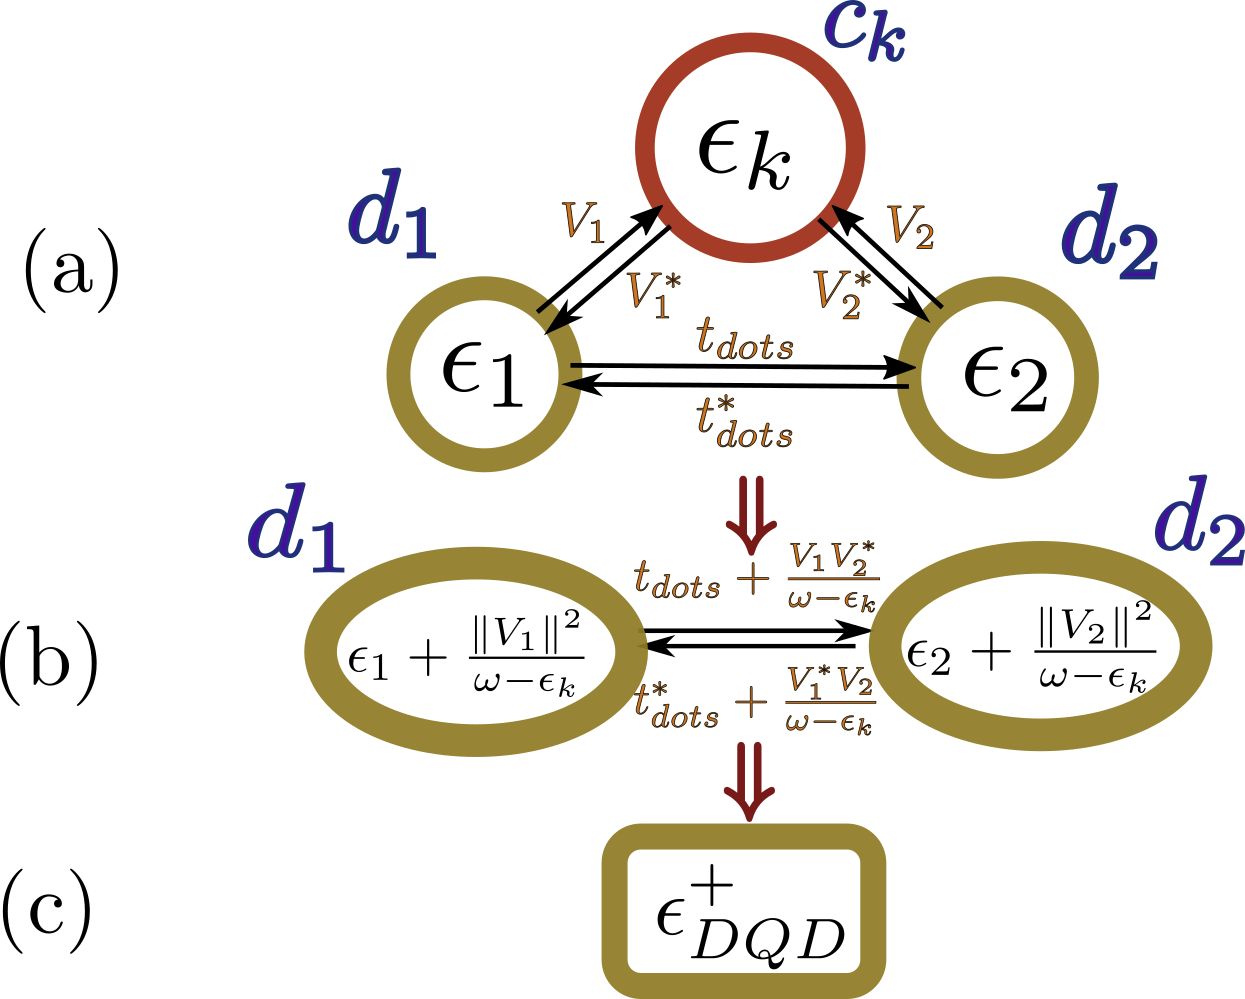
\includegraphics[scale=0.3]{IMAGES/Graphs/DQD-Pro.png}
    \caption{ Graph representation of Gauss-Jordan elimination a) Graph $\GDQD$ b) After the elimination of vertex $c_k$, the energies of dots $d_1$ and $d_2$, and the coupling parameter are changed. c) After Gaussian elimination of dot $2$ the energy of the remaining dot $\epsilon_DQD^+$ represents the transport information through $d_1$ of the entire DQD. \protect\Source{By the author.}}
    \label{fig:graphDQD}
\end{figure}


The algorithm consists in the following. Each step of Gauss-Jordan elimination leads to a new graph with different energies and couplings. The elimination of a row and column is equivalent to pop the corresponding vertex in the graph. For instance, lets eliminate the first row and column of the matrix in \eqref{eq:MatrixDQD}. For it we just need to subtract the rank-$1$ matrix with the same first row and first column
\begin{align}
       & \left[\begin{array}{ccc}
    \omega-\epsilon_{k} & -V_{2} & -V_{1}\\
    -V_{2}^{*} & \omega-\epsilon_{2} & -t_{dots}\\
    -V_{1}^{*} & -t_{dots}^{*} & \omega-\epsilon_{1}
    \end{array}\right]-\left[\begin{array}{ccc}
    \omega-\epsilon_{k} & -V_{2} & -V_{1}\\
    -V_{2}^{*} & \frac{V_{2}^{*}V_{2}}{\omega-\epsilon_{k}} & \frac{V_{2}^{*}V_{1}}{\omega-\epsilon_{k}}\\
    -V_{1}^{*} & \frac{V_{2}V_{1}^{*}}{\omega-\epsilon_{k}} & \frac{V_{1}^{*}V_{1}}{\omega-\epsilon_{k}}
    \end{array}\right] \\ &= \left[\begin{array}{ccc}
    0 & 0 & 0\\
    0 & \omega-\epsilon_{2}-\frac{V_{2}^{*}V_{2}}{\omega-\epsilon_{k}} & -t_{dots}-\frac{V_{2}^{*}V_{1}}{\omega-\epsilon_{k}}\\
    0 & -t_{dots}^{*}-\frac{V_{2}V_{1}^{*}}{\omega-\epsilon_{k}} & \omega-\epsilon_{1}-\frac{V_{1}^{*}V_{1}}{\omega-\epsilon_{k}}
    \end{array}\right]
    \label{eq:Gauss-Jordan} 
\end{align}

The graph associated to this matrix can be observed in \ref{fig:graphDQD}.b) where operator $c_k$ has been popped out of the graph. It is possible to associate the correction to the the energies and couplings to the possible walks passing through the vertex $c_k$.  For instance $d_1$'s energy $\epsilon_1$ receives an extra-term $\frac{V_{1}^{*}V_{1}}{\omega-\epsilon_{k}}$ representing an additional walk  from $d_1$ to $d_1$ passing through  $c_k$. The same logic can be applied to the other terms coupling terms. The correction to $t_dots$ is $\frac{V_{1}^{*}V_{2}}{\omega-\epsilon_{k}}$ which corresponds to a path from $d_1$ to $d_2$ passing through the popped vertex $c_k$. Note that this term includes the multiplication both couplings with the vertex divided by the difference of $\omega$ with the energy of the vertex. This correspondence between the energy correction and eliminated paths through the graph makes the "popping" process an straightforward task. 

We now proceed to pop vertex $d_2$ which leaves just a single vertex as  shown in \ref{fig:graphDQD}.c). The energy of it can be readily computed with the previous path elimination idea which gives 
\begin{equation}
    \epsilon^+_{DQD}=\epsilon_{1}+\sum_{\mathbf{k}}\frac{V_{1}V_{1}^{*}}{\omega-\epsilon_{\mathbf{k}}}+\frac{\left\Vert t_{dots}+\sum_{\mathbf{k}}\frac{V_{1}V_{2}^{*}}{\omega-\epsilon_{\mathbf{k}}}\right\Vert ^{2}}{\omega-\epsilon_{2}-\sum_{\mathbf{k}}\frac{V_{2}V_{2}^{*}}{\omega-\epsilon_{\mathbf{k}}}},  \label{eq:EnDQD}
\end{equation}
\noindent where we selectively included the $\sum_k$-terms in the places where $k$ appeared. 

As a result of  Gauss-Jordan elimination the linear equation in \ref{eq:MatrixDQD} has evolved into the trivial form 
\begin{equation}
\left[\begin{array}{ccc}
0 & 0 & 0\\
0 & 0 & 0\\
0 & 0 & \omega-\epsilon_{DQD}^{+}
\end{array}\right]\left[\begin{array}{c}
\Green{c_{\mathbf{k}},d_{1}^{\dagger}}\\
\Green{d_{2},d_{1}^{\dagger}}\\
\Green{d_{1},d_{1}^{\dagger}}
\end{array}\right]=\left[\begin{array}{c}
0\\
0\\
1
\end{array}\right].
\end{equation}
The Green function is then 
\begin{align}
\Green{d_{1},d_{1}^{\dagger}}=\frac{1}{\omega -  \epsilon^+_{DQD}} =\left[\left(\omega-\epsilon_{1}-\sum_{\mathbf{k}}\frac{V_{1}V_{1}^{*}}{\omega-\epsilon_{\mathbf{k}}}\right)-\frac{\left(t_{dots}+\sum_{\mathbf{k}}\frac{V_{1}V_{2}^{*}}{\omega-\epsilon_{\mathbf{k}}}\right)\left(t_{dots}+\sum_{\mathbf{k}}\frac{V_{1}V_{2}^{*}}{\omega-\epsilon_{\mathbf{k}}}\right)^{*}}{\omega-\epsilon_{2}-\sum_{\mathbf{k}}\frac{V_2V_{2}^{*}}{\omega-\epsilon_{\mathbf{k}}}}\right]^{-1}. \label{eq:SumSolGreen} 
\end{align}
This Green function will be very important in the following chapters where we will compare its behavior with the green function of a Majorana mode. 
% the inverse of the green function $G_{d_1d^\dagger_1}$. The final result is then 

% \begin{equation}
    % \Green{d_{1},d_{1}^{\dagger}}=\left[\left(\omega-\epsilon_{1}-\frac{V_{1}V_{1}^{*}}{\omega-\epsilon_{\mathbf{k}}}\right)-\frac{\left(t_{dots}+\frac{V_{1}V_{2}^{*}}{\omega-\epsilon_{\mathbf{k}}}\right)\left(t_{dots}+\frac{V_{1}V_{2}^{*}}{\omega-\epsilon_{\mathbf{k}}}\right)^{*}}{\omega-\epsilon_{2}-\frac{\Gamma_{2}^{2}}{\omega-\epsilon_{\mathbf{k}}}}\right]^{-1}. \label{eq:solGreen}
% \end{equation}

% Just one additional correction. Remember that every term including $\epsilon_k$ is summing over all possible energies in the momentum space. We avoided this sum during the process to avoid carrying this term during the process. But it is important to include it know.  

% \begin{equation}
%      \Green{d_{1},d_{1}^{\dagger}}=\left[\left(\omega-\epsilon_{1}-\sum_{\mathbf{k}}\frac{V_{1}V_{1}^{*}}{\omega-\epsilon_{\mathbf{k}}}\right)-\frac{\left(t_{dots}+\sum_{\mathbf{k}}\frac{V_{1}V_{2}^{*}}{\omega-\epsilon_{\mathbf{k}}}\right)\left(t_{dots}+\sum_{\mathbf{k}}\frac{V_{1}V_{2}^{*}}{\omega-\epsilon_{\mathbf{k}}}\right)^{*}}{\omega-\epsilon_{2}-\sum_{\mathbf{k}}\frac{\Gamma_{2}^{2}}{\omega-\epsilon_{\mathbf{k}}}}\right]^{-1}. \label{eq:SumSolGreen}
% \end{equation}

\subsection{Graph Algorithm \label{sec:Algorithm}}

In this part we summarize the steps of the graph algorithm in order to apply them later to more complicated systems:
\begin{enumerate}
    \item Computing the transport equations with the second term fixed in the creation operator of  $d^\dagger$.
     \item  Writing the  graph associated to the transport system. The vertexes are the operators in the first site of the of the green functions. Energies and couplings are associated to the vertex and edge numbers of the graphs respectively.  
    \item Popping the vertexes of the graph. Each vertex popping involves the following steps.
    \begin{enumerate}
        \item Computing the extra-terms in the energies and couplings based on the walks passing through the popped vertex.
        \item Eliminating this vertex from the graph. 
        \item Iterating till there is only the vertex $d$.
        \end{enumerate}
    \item The energy in the remaining vertex $d$ is $\epsilon_d = \frac{1}{\omega -\Green{d,d\dagger}}$ .
\end{enumerate}

This algorithm will be our main method to find the green function and therefore the density of states of any interacting system. 


% However this method lacks of any useful intuition that could help us  to  solve more complex systems. This remarks the  importance of pursuing alternative methods. \\




% Let $v_1$ and $v_2$ be two operators in $\GDQD$. If an operator $v_2$ appears in the right side of the transport equation for vertex $v$, the graph will have  a directed edge from $v_2$ to $v_1$. A weight is assign to this edge given by the coefficient of $v_2$ in $v_1$'s transport equation. Note that this relation is reciprocal since the Hamiltonian is hermitian. Hence if there is an arrow from $v_1$ to $v_2$ with weight $t$, then there there will be an opposite arrow from $v_2$ to $v_1$ with weight $t^*$. e.g. In this case, the tree operators  $d_{1\downarrow},d_{2},c_{\boldsymbol{k}}$ are connected. The weights of these connections are observed in \ref{fig:graphDQD}.\\



% Now, the Green functions $\Green{d_{1},d_{1}^{\dagger}}$ will always have the form $\frac{1}{\omega-E} $ where $E$ is an energy. This form is also observed in \ref{eq:solGreen}.  Looking at equation \ref{eq:green1},  observe that if $\Green{d_{2},d_{1}^{\dagger}}$ and $\sum_{\mathbf{k}}\Green{c_{\mathbf{k}},d_{1}^{\dagger}}$ are multiples of $\Green{d_{1},d_{1}^{\dagger}}$ (i.e $\Green{d_{2},d_{1}^{\dagger}}=\eta_{2}\Green{d_{1},d_{1}^{\dagger}},\Green{c_{\mathbf{k}},d_{1}^{\dagger}}=\eta_{\boldsymbol{k}}\Green{d_{1},d_{1}^{\dagger}})$ , the result for $\Green{d_{1},d_{1}^{\dagger}}$ will be 
% \begin{equation}
%     \Green{d_{1},d_{1}^{\dagger}}=\frac{1}{\omega-\epsilon_{1}-\sum_{\boldsymbol{k}}V_{1}^{*}\eta_{\boldsymbol{k}}+t_{dots}\eta_{2}}.
% \end{equation}

% Hence to obtain $\Green{d_{1},d_{1}^{\dagger}}$ we need to find $\eta_{\boldsymbol{k}}$ and $\eta_{2}$. Now note from equation \eqref{eq:green2} that $\left(\omega-\epsilon_{\boldsymbol{k}}\right)\eta_{\boldsymbol{k}}=V_{1}+V_{2}\eta_{2}$

% \begin{equation}
% \Green{d_{1},d_{1}^{\dagger}}=\frac{1}{\omega-\epsilon_{1}-\sum_{\boldsymbol{k}}\frac{V_{1}^{*}V_{1}}{\omega-\epsilon_{\boldsymbol{k}}}+V_{1}^{*}V_{2}t_{dots}\eta_{2}\eta_{2}}    
% \end{equation}


% Now, probably at this point you might already know what is happening here. Basically the energy $E$ represents the sum of all possible transitions in the graph that start and finish at $d_{1}$ . The first term is $\epsilon_{1}$, which is the energy of dot $1$. The next term is $\frac{V_{1}^{*}V_{1}}{\omega-\epsilon_{\boldsymbol{k}}}$ which represents the transition $d_{1}\rightarrow c_{k}\rightarrow d_{1}$. Note that $\frac{V_{1}^{*}V_{1}}{\omega-\epsilon_{\boldsymbol{k}}}$ is basically the energy needed to go from $d_{1}$ to $c_{\boldsymbol{k}}$ and coming back divided by the energy "cost" of passing through $c_{\boldsymbol{k}}$ which is $\omega-\epsilon_{\boldsymbol{k}}$. The sum over $\textbf{k}$ can be ignored in this analysis. Now we can then explain why the last term in \eqref{eq:solGreen} is 
% \begin{equation}
%     \frac{\left(t_{dots}+\sum_{\mathbf{k}}\frac{V_{1}V_{2}^{*}}{\omega-\epsilon_{\mathbf{k}}}\right)\left(t_{dots}^{*}+\sum_{\mathbf{k}}\frac{V_{1}^{*}V_{2}}{\omega-\epsilon_{\mathbf{k}}}\right)}{\omega-\epsilon_{2}-\sum_{\mathbf{k}}\frac{\Gamma_{2}^{2}}{\omega-\epsilon_{\mathbf{k}}}}. \label{term}
% \end{equation}

% Firs note that $\left(t_{dots}+\sum_{\mathbf{k}}\frac{V_{1}V_{2}^{*}}{\omega-\epsilon_{\mathbf{k}}}\right)$ is the energy needed to go from $d_{1}$ to $d_{2}$. This could occur by passing through $c_{\boldsymbol{k}} \ \left(\sum_{\mathbf{k}}\frac{V_{1}V_{2}^{*}}{\omega-\epsilon_{\mathbf{k}}}\right)$ or going directly to $d_ 2$ $\left(t_{dots}\right)$. The term is multiplied by $\left(t_{dots}^{*}+\sum_{\mathbf{k}}\frac{V_{1}^{*}V_{2}}{\omega-\epsilon_{\mathbf{k}}}\right)$ which represents the opposed transition from $d_{2}$ to $d_{1}$.  Finally, we  divide this by the cost of passing through $d_{2}$ and $c_{\boldsymbol{k}}$. This is basically to multiply by the green function taking the point $d_{1}$ out of $\GDQD$ . This green function is


% \begin{equation}
%     \GreenG{d_2,d_2^\dagger}{\GDQD-d1}= \frac{1}{\omega-\epsilon_{2}-\sum_{\mathbf{k}}\frac{\Gamma_{2}^{2}}{\omega-\epsilon_{\mathbf{k}}}}.
% \end{equation}
% where $\GreenG{d_2,d_2^\dagger}{\GDQD-d_1}$ is the green function of $d_2,d_2^\dagger$ in the smaller graph $\GDQD-d_1$. 

% The last equation not only explains the meaning of term \eqref{term} in equation \eqref{eq:solGreen}. It also gives us an iterative method to find the green function. To understand this, note that the solution in \eqref{eq:solGreen} can also be written as 

% \begin{equation}
% \left( \GreenG{d_{1},d_{1}^{\dagger}}{\GDQD} \right) ^{-1}= \omega - \epsilon_1- \sum_\textbf{k} E_{d_1c_k}^{\GDQD-d_2} \GreenG{c_\textbf{k}c^\dagger_\textbf{k}}{\GDQD-d_2-d_1}  - E_{d_1d_2}^{\GDQD} \GreenG{d_2,d_2^\dagger}{\GDQD-d_1} . \label{eq:solGreen2}
% \end{equation}
% Where $E_{d_1c_k}^{\GDQD-d_2} = \sum_{\boldsymbol{k}}\frac{V_{1}^{*}V_{1}}{\omega-\epsilon_{\boldsymbol{k}}} $  represents the accumulated energy of going from $d_1$ to $c_k$ and coming back. The upper-index $\GDQD-d_2$ represents that at this step the second dot is ignored. Similarly $E_{d_1d_2}^{\GDQD}$ is the numerator of \eqref{term}. It represents the energy accumulated in at going from $d_1$ to $d_2$. Since this time no point is ignored, the upper-index remains as $\GDQD$. \\

% Now the amazing thing about the last equation is that it decomposes the green function $\GreenG{d_{1},d_{1}^{\dagger}}{\GDQD}$  into green functions of smaller graphs. This gives an iterative process to compute green functions using induction in graphs .  Now, as you might see, the complexity of these green functions reduce strongly after a single point is removed out of the graph . This makes green function computation a pretty simple task using the graph method. 

% \Jesus{I promise a real proof of this fact to be included in the abstract. The idea is using induction in graphs  \ref{sec:AbsGraphmethod}. }

\subsection{Ballistic transport in a  double quantum dot \label{sec:GreedDQD}}

In this subsection we describe the remaining steps to extract the density of states of the double quantum dot from the Green function \ref{eq:SumSolGreen}. We will plot the results and observe the evolution of the DOS while tuning the parameters of the model. 

First note that equation \eqref{eq:SumSolGreen} depends on the term $\sum_{\boldsymbol{k}}\frac{V_{i}^{*}V_{j}}{\omega-\epsilon_{\boldsymbol{k}}}$ which describes the broadening of the DOS when the QD enters in contact with the lead. This broadening is usually named $\Gamma_i=V_{i}^{*}V_{i}$ (Or $\Delta$ depending on the text book). 
% $$-\Gamma_i = \sum_{\boldsymbol{k}}\frac{V_{1}^{*}V_{1}}{\omega-\epsilon_{\boldsymbol{k}}}. $$
In general $V_i$  is a function of $\textbf{k}$. However, in the limit of flat-band we can assume that $V_i $ is constant. Therefore, it is enough to integrate
\begin{equation}
    \sum_{\boldsymbol{k}}\frac{1}{\omega-\epsilon_{\boldsymbol{k}}+is}=\int_{-D}^{D}\frac{d\epsilon_{\boldsymbol{k}}}{\omega-\epsilon_{\boldsymbol{k}}+is}=-\ln\left(\frac{D-\epsilon_{\boldsymbol{k}}+is}{-D-\epsilon_{\boldsymbol{k}}+is}\right)\xrightarrow[D\rightarrow\infty]{}-i , 
\end{equation}
\noindent where we assumed that there is a maximum  energy cutoff $D$ going to infinity in the wide-band limit. Hence 
\begin{equation}
   -i\Gamma_i = \sum_{\boldsymbol{k}}\frac{V_{i}^{*}V_{i}}{\omega-\epsilon_{\boldsymbol{k}}}.
\end{equation}



We can replace this in equation \eqref{eq:SumSolGreen} to obtain the real expression for the green function $\Green{d_1,d_1^\dagger}$. The terms of the form $V_1V_2^*$ can be replaced for $\sqrt{\Gamma_1\Gamma_2}$, supposing there is no additional complex phase.

Now, remember from \eqref{eq:Density of States} that the DOS $\rho$ depends on the imaginary factor of the Green Function $\Green{d_1,d_1^\dagger}$. This term depends in the broadening $\Gamma$. If $\Gamma = 0$ the density of states will be $0$ as well. At any other case, one of the dots should be attached to the lead. Let $\Gamma_1$ be the broadening of this dot. We will take $\Gamma_1$ as our natural unit for the rest of this thesis.  

In \ref{fig:GreenDQD} we can observe the evolution of the Density of States under certain processes. Each plot includes an inset showing the model applied to the figure. The coupling in purple indicates the tuning variable. We set $e_1 = e_2 = 0$ so that both dots satisfy PHS. The primary results are the 

   % ----------------SUPER FIGURE ---------------------------
    \begin{figure}[t]
        \centering
         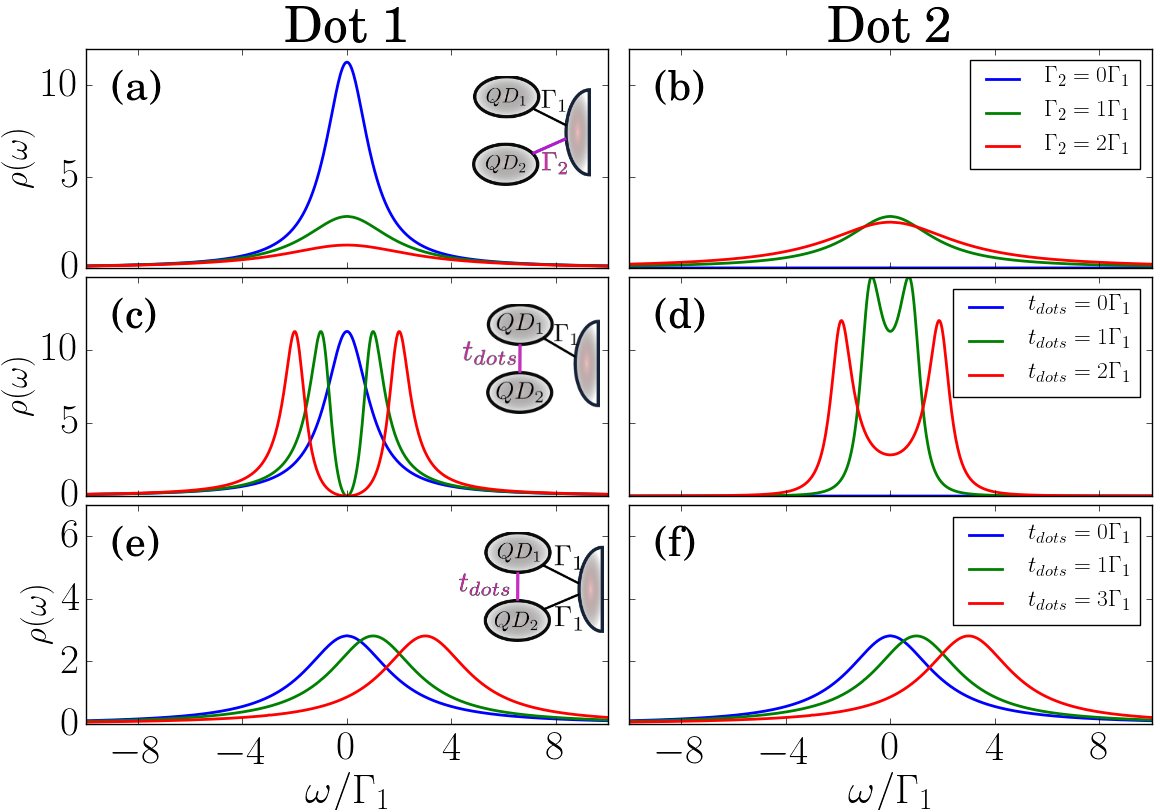
\includegraphics[scale=0.47]{IMAGES/DQD/Non-interacting.png}
         \caption{\label{fig:GreenDQD} Evolution of the density of states at each QD (Left: dot 1, Right: dot 2) at three distinct arrangements of DQD-lead coupling. The inset at the first column depicts the type of coupling. The purple line represents the tuning variable. The energy unit is $\Gamma_1$. $e_1 =e_2 =0$ in all arrangements. (a),(b) The lead is connected to both QDs. Tuning variable: $\Gamma_2$. (c)(d) Indirect coupling of the second dot through dot one. Tuning variable: $\_{dots}$. (e)(f) Triangular coupling. Tuning variable: $t_{dots}$.  
         \protect\Source{ By the Author  }}
    \end{figure}
% ----------------SUPER FIGURE ---------------------------


\begin{enumerate}
    \item \textbf{Coupling QD2. \ref{fig:GreenDQD}(a)(b):}  At $\Gamma_2=0$  the second dot is decoupled, hence the first dot's DOS is the same of a single dot case. The maximum height is achieved at  $\rho \pi \Gamma_1 =1$ and the width of this peak is about  $\Gamma_1$, just as in Figure \ref{fig:specDots}. When the second dot is attached $\Gamma_2 >0$ the density of states is divided between both dots. At $\Gamma_1 = \Gamma_2$ the DOS at the Fermi energy is equal to $\frac{1}{4\pi\Gamma}$ for both dots. For higher values of $\Gamma_2$ the DOS in the second dot is higher than in the first one.  
    
 

    \item \textbf{Indirect Coupling of QD2. \ref{fig:GreenDQD}(c)(d):} This is case is interesting. When the second dot is connected indirectly through the first dot, quantum inference splits the central peak in two new states. We will observe later that in the interacting case this procedure can also destroy the Kondo signature. Note that the higher the coupling $t_{dots}$ is, the greater is the gap between the states. We will usually take $t_{dots} = 2\Gamma_1$ to make these gap more visible in the NRG simulations. 
    % This has interesting consequences when combined with Majorana physics.
    \item \textbf{Breaking Particle Hole Symmetry. \ref{fig:GreenDQD}(e)(f):}
    Suppose we have $\Gamma_2 = \Gamma_1$. The "triangular connections" break Particle Hole Symmetry. The central peak is displaced to the positive part of the spectrum. We will avoid this situation during this project, because because PHS-breaking  will prevent the Majorana to tunnel inside the DQD. Hence, this model won't lead to any interesting result on Majorana manipulation. 
\end{enumerate}



% \begin{figure}[H]
%      \centering
    
%      \subfloat[Attaching QD2 to the lead \label{fig:DQD-G2}]{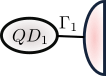
\includegraphics[scale=0.6]{IMAGES/DQD/g1g2-m.png}} \\
%     \subfloat[Indirect connection of QD2 \label{fig:DQD-tdots}]{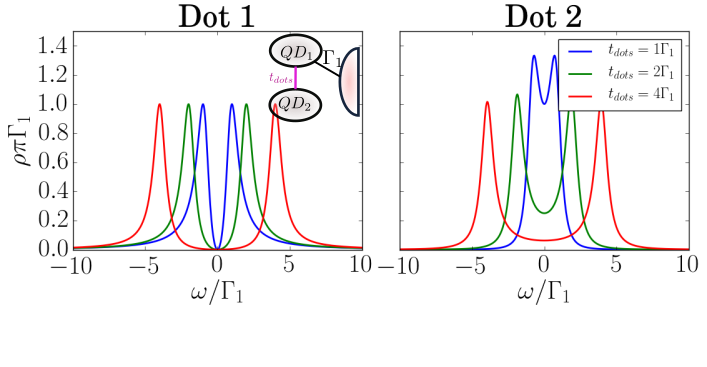
\includegraphics[scale=0.6]{IMAGES/DQD/tdots-m.png}}\\
%     \subfloat[Breaking PHS with triangular connection \label{fig:DQD-PHS}]{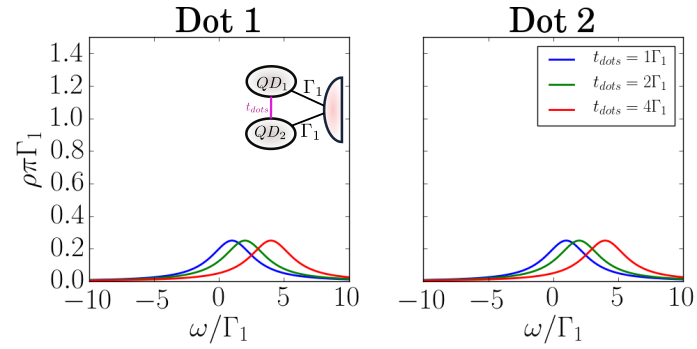
\includegraphics[scale=0.6]{IMAGES/DQD/phs-m.png}}
%      \caption{\label{fig:GreenDQD} For the tree cases we considered $e_1 =e_2 =0$. The inset shows the set-up. At each case the purple coupling shows the tuning variable. \protect\Source{ By the Author  }}
% \end{figure}














% ------------------------------------------NRG----------------------
% ---------NRG-------------------------------------------------------
% ------------------ NRG --------------------------------------------
% -----------------------------------------------------NRG------------



\section{The Numerical Renormalization Group\label{sec:The-Numerical-Renormaliztion} (NRG) }

\subsection{From the Renormalization Group to the Wilson's Chain \label{subsec:Logarithmic}}

%-------------------------------------------------------
\begin{figure}[hbt]
\centering
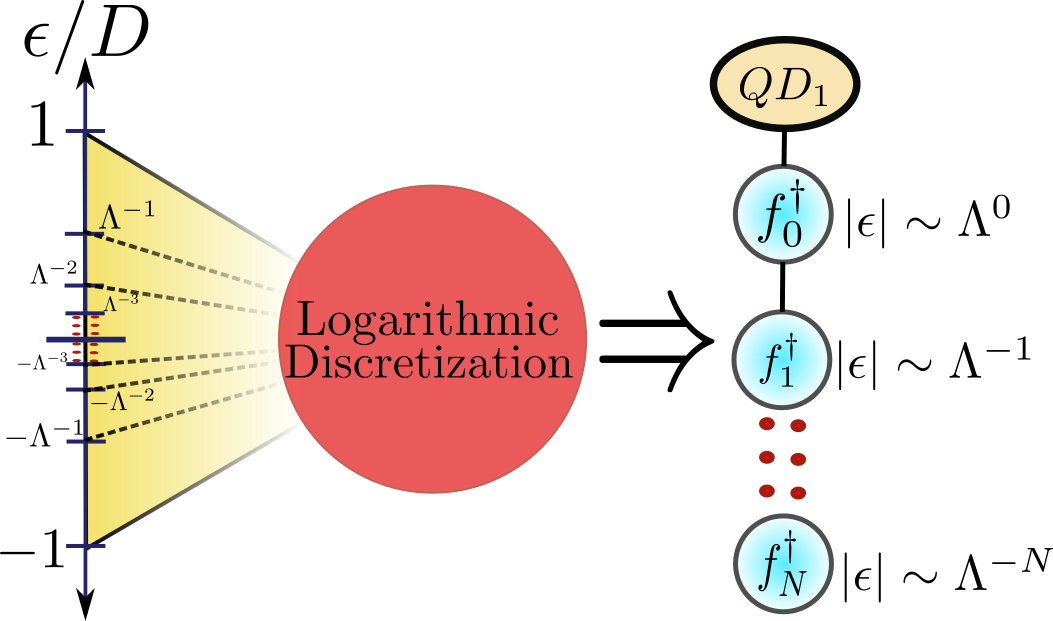
\includegraphics[scale=0.45]{IMAGES/DQD/NRG-Final.png}\caption{\label{fig:Discretization}.
Energy interval discretization. \protect\Source{ By the Author  } }
\end{figure}
%--------------------------------------------------

 The real meaning of divergent logarithmic term in the resistivity predicted by Kondo is that important contributions at low-energy scales caused by the strong quantum correlations in the system are being neglected by perturbation theory. This problem can be solved by introducing ideas from renormalization group theory. A renormalization approach is more adequate for this type of problem since it assigns an appropriate effective Hamiltonian to each scale of temperature. This provides a more accurate representation of the increasing density of correlated states appearing close the Fermi energy. 

In renormalization group theory, the Hamiltonian transformations are performed by an operator $\mathcal{T}$ that represents an endomorphism in the space of operators. $T$ generates the semigroup  $\{ 1, \mathcal{T} , \mathcal{T}^2 , \ldots \}$, that defines a complete set of transformations   % transformation of the form
$$ \mathcal{T}[H_0] = H_1, \  \mathcal{T}[H_1] = H_2, \ldots , \mathcal{T}[H_N] = H_{N+1} , \ldots$$
\noindent If $\mathcal{T}$ is a contracting map  \footnote{ Let $\mathcal{O}$ be a set of operators, then $T$ is a contracting map if $\mathcal{T}[\mathcal{O'} ] \subset \mathcal{O'}$ for every $\mathcal{O'} \subset \mathcal{O}$ .} then it is known that this set of operations should eventually lead to a fix point $ \mathcal{T}^N[H] \xrightarrow{N\rightarrow\infty} H*$ such that $\mathcal{T}[H*] = H*$. In numerical simulations, $N $ will only increase up to a value where $H_N$ is close enough to the fix point $H*$ so that no new significant contributions to the Hamiltonian are obtained. For the purposes of this project, taking $N = 51$ will be enough  for the NRG code to converge. 

%Maybe the most important characteristic of the Kondo effect is that leading contributions to the conductivity are caused by strong correlations with the conduction band appearing at low energy scales. This is the reason of the divergent logarithmic term in the Kondo resistivity. 

In the 1970's G.Wilson used this theory to create the famous Numerical Renormalization Group (NRG) \citep{bulla_numerical_2008,wilson_renormalization_1975,krishna-murthy_renormalization-group_1980}. His main idea was to perform a logarithmic discretization of the conduction band in the lead as shown in \ref{fig:Discretization}.(a). Taking into account that the leading contributions to the conductance occur at states close to the Fermi energy $\omega = 0$, we can define a cut-off $( \vert \omega \vert < D)$ so that the rest at higher contributions are not relevant.Then we use D to rescale the energy interval. As you can observe in the figure, the QD is coupled to all these energy states at the same time. The logarithmic discretization gives more relevance to the low energy scales by assigning a different Hamiltonian coupling to each one of them. To complete this idea, the NRG code maps the Hamiltonian of the QD-lead system to the Wilson's chain shown in \ref{fig:Discretization}(b). A detailed description of this map is included in the Appendix \ref{sec:LogarithmicDisc}.

After these steps we obtain a chain Hamiltonian of the form 

\begin{equation}
H=H_{d}+D\sum_{\sigma}\Biggl[\sqrt{\frac{2\Gamma}{\pi D}}\left(d_{\sigma}^{\dagger}f_{0\sigma}+f_{0\sigma}^{\dagger}d_{\sigma}\right)+\frac{1}{2}\left(1+\Lambda^{-1}\right)\sum_{n=0}^{\infty}\Lambda^{\frac{-n}{2}}\xi_{n}\left(f_{n\sigma}^{\dagger}f_{n+1,\sigma}+f_{n+1\sigma}^{\dagger}f_{n\sigma}\right)\Biggr].\label{eq:chain-Hamiltonian}
\end{equation}


In the flat-band approximation the parameters $\xi_{n}$ can be obtained analytically \citep{bulla_numerical_2008}
\[
\xi_{n}=\frac{1-\Lambda^{-n-1}}{\left(1-\Lambda^{-2n-1}\right)^{\frac{1}{2}}\left(1-\Lambda^{-2n-3}\right)^{\frac{1}{2}}}.
\]


%The formal recursive-solution of this problem can be found in \citep{bulla_numerical_2008}. 
From equation \prettyref{eq:chain-Hamiltonian}  we define the following set of Hamiltonians

\begin{equation}
H_{N+1}=T\left[H_{N}\right]=\Lambda^{-\frac{1}{2}}H_{N}+\xi_{N}\left(f_{N+1,\sigma}^{\dagger}f_{N,\sigma}+f_{N,\sigma}^{\dagger}f_{N+1,\sigma}\right), \label{eq:NRG-Renormalization}
\end{equation}

with 
\begin{equation}
H_{-1} := \frac{2 H_d}{1+\Lambda^{-1}}.
\end{equation}

%Then the initial Anderson model can be recovered in the limit 
%\begin{equation}    
%H = \lim_{N \rightarrow \infty } \frac{1+\Lambda^{-1}}{2}\Lambda^\frac{ N-1 }{2} H_N
%\end{equation}
The Renormalization Group transformation $\mathcal{T}$ can be defined as 

$$\mathcal{T}^N H_{-1} =  \frac{1+\Lambda^{-1}}{2}\Lambda^\frac{ N-1 }{2} H_N$$

Note that in the limit $\xrightarrow{N\rightarrow\infty}$ we should recover the initial Anderson Hamiltonian. In addition, note that the leading coefficients of the contributions to each Hamiltonian $H_N$ are given by 
\[
\Lambda^{\frac{-N}{2}}\xi_{N}\xrightarrow{N\rightarrow\infty}\frac{\Lambda^{\frac{-N}{2}}\left(1-\Lambda^{-N}\right)}{1-\Lambda^{-2N}}\sim\frac{\Lambda^{\frac{-N}{2}}}{1+\Lambda^{-N}},
\]
\noindent which decays exponentially with the length of the chain. Therefore, we may thing that at some point these new contributions will be so small that the that the map $\mathcal{T}$ will eventually converge. Formally the theory regarding the NRG convergence is to complex for this thesis. However the results show that the operator that trully converges is $\mathcal{T}^2$ and not $\mathcal{T}$\cite{krishna-murthy_renormalization-group_1980}. This has important consequences, for instance the convergence of the code has to be analyzed on odd and even values of $N$ separately. 

To this point the expression \prettyref{eq:chain-Hamiltonian} and the derived limit of $H_N$ to the Anderson Hamiltonian are exact. The first approximations arrive in the following step which include an iterative diagonalization of the Hamiltonian.
 
 \subsection{Iterative Diagonalization \label{subsec:IterativeDiag}}

\begin{figure}[bt]
\centering
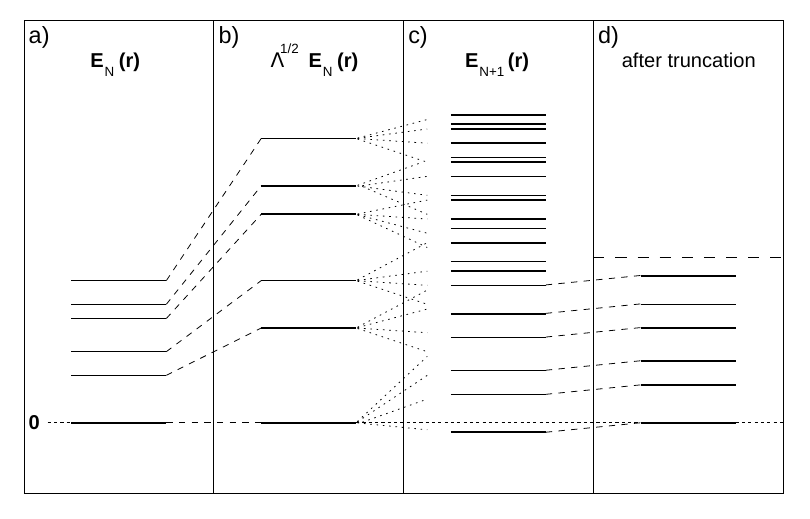
\includegraphics[scale=0.5]{IMAGES/DQD/cutting.png}
\caption{ \label{fig:IterativeDiagonalization} Iterative diagonalization process. \protect\Source{ \cite{wilson_renormalization_1975} } }
\end{figure}


 This diagonalization starts with the impurity/dot Hamiltonian $H_{-1}$, which must be written in matrix form according to a defined basis. The other steps can be defined by induction.  Suppose that the spectrum of $H_{N}$ is diagonal on a given basis. Then the NRG code performs each of the following steps:

\begin{enumerate}
 	\item Rescaling the spectrum of $H_{N}$ by $\Lambda^{\frac{1}{2}}$ as defined in \ref{eq:chain-Hamiltonian}. \ref{fig:IterativeDiagonalization} (a)$\rightarrow$(b).
 	\item Adding the next step of the chain to form $H_{N+1}$ and diagonalizing the new Hamiltonian such that $H_{N+1} = U_{N+1}^\dagger D_{N+1} U_{N+1}$ . After this step, each of the eigenstates of $H_{N}$ will spit in up to $4$ new energy states (probably degenerate) determined by the new coupling with the  $N+1$ site basis ${\vert 0 \rangle, \vert \up \rangle, \vert \dw \rangle, \vert \up \dw \rangle}$.  \ref{fig:IterativeDiagonalization} (b)$\rightarrow$(c).
 	\item Shifting the spectrum by a certain dephase factor such that the $0$ of energy is always the ground state.  \ref{fig:IterativeDiagonalization} (c)$\rightarrow$(d).
 	\item Numerical cutting: If the number of states in the system exceeds a definite number (1000 in this thesis) the exceeding higher energy states are neglected.\footnote{ This step must be performed carefully to preserve the symmetries of the system. If two states are entangled and one of them is eliminated and the other is not, the program could lead to misleading results. Further discussions to solve this problem are presented in the symmetry subsection.  }. \ref{fig:IterativeDiagonalization} (c)$\rightarrow$(d).
 	\item Rotating operators $f_{N,\sigma}$  by $ U_N f_{N,\sigma} U_N^\dagger$ to start the next operation.
\end{enumerate}

The final outcome of this operations will be the complete spectrum of the Anderson model at each energy level. However we still need to talk about an important speed-up to the code obtain when considering the symmetries of the system. 

\subsection{Symmetries \label{subsec:Syms}}

The symmetries of the initial Hamiltonian take a very important role in this iterative diagonalization. Lets suppose that the initial Hamiltonian $H_d$ has certain symmetries classified by the quantum number $S$ . Then $H_d$ can be written can be represented in block Hamiltonians over a basis of the form $\vert S, i\rangle$. A diagnolization process of an square matrix with $L$ rows usually has an square order proportionate to the number of entries $\mathcal{O}\sim L^2$. However, if the matrix is organize in blocks of length $N_j$  such that $\sum_j L_j = L$, then the order of diagonalization will be around $\sum_j L_j^2  $ which is in general much smaller than $(\sum_j L_j)^2 L^2$. Therefor the block diagonalization provides important numerical advantages to the algorithm. 

To keep this speed-up we must preserve this symmetry structure for the rest of the algorithm. For it, we first need to verify that the picked symmetry also commutes with the hopping terms in the chain Hamiltonian. If so, for each step  $N$ of the NRG algorithm we will have that the $H_N$ Hamiltonian can be written in a block diagonal form with basis 
$\vert S_N, i_N\rangle$. Then it is necessary to define transition rules from the quantum numbers $S_N$ to $S_{N+1}$. By doing this, we assure that the block architecture is transmitted through the entire algorithm, hence reducing the computational time significantly at each step of the NRG chain. 


In the following subsection we will give examples of this symmetry propagation in the example a quantum dot attached to a metallic lead. 




% This block structure simplifies the diagonalization process since the algorithm can diagonalize each block one by one.  This is numerically favorable since the diagonalization of a quadratic matrix  

% takes a quadratic order $n^2$ in a fully entry matrix. Keeping the blocks during the entire NRG 

% Since a numerical diagonalization algorithm have quadratic order $n^2$, it is numerically favorable

%In \ref{sec:Kondo} we observed that the Kondo resistivity had a logarithmic contribution which led to a huge trouble when describing energies bellow the Kondo temperature. This logarithmic term has a  especial meaning which is that the lower energy scales are also relevant. Thus, to solve the Kondo problem it was necessary to create a theory that could efficiently integrate the contributions from all energy scales. In the 1970's G.Wilson created a numerical method that mixed ideas from scalability and renormalization group. This method proofed to be the most efficient form to understand the Kondo effect as well as other impurity problems described by the Anderson Model. 

%Wilson's idea was to discretize the conductance band logarithmically in energy in 
 
%In the 1970's G.Wilson created a numerical method to solve the Anderson model . This method receives the name of Numerical Renormalization Group (NRG) \citep{bulla_numerical_2008,wilson_renormalization_1975,krishna-murthy_renormalization-group_1980}.



% It consists of three basic steps :
% \begin{enumerate}
% \item To perform a numerical discretization of the energy spectrum in logarithmic intervals. 
% \item To map the discretized model onto a semi-infinity chain Hamiltonian. 
% \item  To diagonalize iteratively the chain hamiltonian . 
% \end{enumerate}

% The final result will be the spectrum of the Hamiltonian. Other important properties of the material such as density of states, conductivity, specific heat, susceptibility can also be computed. On this project we are mainly interested in the Density of States (DOS). The method used to compute the DOS is the Density Matrix numerical renormalization Group (DM-NRG). A complete description of this algorithm will be given in the following sections.  \\

% For now, we proceed to describe how the NRG is applied to solve the Anderson model in a QD:\\

% \Jesus{I still need to do a long revision to this section. Probably I will send most of the computations to the abstract and leave a summary of NRG and its advantages in the main text.}







%\begin{figure}[h]
%\centering
%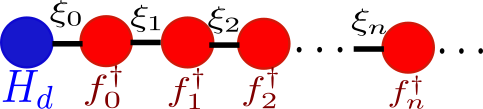
\includegraphics[scale=0.5]{IMAGES/NRGchain.png}\caption{\label{FigNRG-chain} Chain-Hamiltonian describing the Anderson model.
%The chain starts at the initial dot hamiltonian $H_{d}$. The $f_{m}^{\dagger}$'s
%are the creation operators at the $n^{\mbox{th}}$-site of the chain.
%The $\xi_{n}$'s describe the magnitude of the interaction between
%consecutive sites. }
%\end{figure}




\subsection{Iterative diagonalization in a single QD Hamiltonian \label{subsec:QD-Diag} }

Now that we have an iterative representation of the Anderson Model
Hamiltonian \prettyref{eq:chain-Hamiltonian}, lets take a look to
how the NRG code would work for a QD. We start with the dot Hamiltonian.
(Since the $D$ term is always present as a normalizing factor, we
are going to avoid this term in future computations and suppose that
we are working with unit-less variables $\epsilon_{d},\ U$ and $\Gamma':=\sqrt{\frac{2\Gamma}{\pi D}}$
).
\begin{equation}
H_{d}=\frac{1}{D}\left(\epsilon_{d}+\frac{U}{2}\right)d_{\sigma}^{\dagger}d_{\sigma}+\frac{U}{2D}(d_{\sigma}^{\dagger}d_{\sigma}-1)^{2}.\label{eq:DotHam}
\end{equation}


Now observe that hamiltonian \ref{eq:DotHam} already has a
diagonal form in the base $\left\{ \vert\uparrow\!\downarrow\rangle,\vert\uparrow\rangle,\vert\downarrow\rangle,\vert0\rangle\right\} $
\[
H_{d}=\frac{1}{D}\left[\begin{array}{cccc}
2\epsilon_{d}+\frac{3U}{2} & 0 & 0 & 0\\
0 & \epsilon_{d}+\frac{U}{2} & 0 & 0\\
0 & 0 & \epsilon_{d}+\frac{U}{2} & 0\\
0 & 0 & 0 & \frac{U}{2}
\end{array}\right].
\]


Lets define $H_{-1}=\Lambda^{\frac{-1}{2}}H_{d}.$ Adding the first
chain interaction to $H_{d}$ we obtain a new Hamiltonian of the form 

\begin{equation}
H_{0}=\Lambda^{\frac{1}{2}}H_{-1}+\Gamma'\left(d_{\sigma}^{\dagger}f_{0\sigma}+f_{0\sigma}^{\dagger}d_{\sigma}\right).\label{eq:H0fromH-1}
\end{equation}


The Hilbert space for this Hamiltonian has to be extended to include
the $4$ degrees of freedom of the $f_{0\sigma}^{\dagger}$ particles
which are also given by $\left\{ \vert\uparrow\!\downarrow\rangle,\vert\uparrow\rangle,\vert\downarrow\rangle,\vert0\rangle\right\} $.
Therefore the total Hilbert space for $H_{0}$ is given by a base
of the form 
\[
\vert s_{1}\rangle\vert s_{2}\rangle:=\vert s_{1}\rangle\otimes\vert s_{2}\rangle\mbox{ with }\vert s_{i}\rangle\in\left\{ \vert\uparrow\!\downarrow\rangle,\vert\uparrow\rangle,\vert\downarrow\rangle,\vert0\rangle\right\} .
\]


We obtain an space of dimension $4\times4=16.$ Now, before adventuring
to write the Hamiltonian for $H_{0}$ as a $16\times16$-matrix note
that $H_{-1}$ preserves particle number $\mathcal{N}$ and the total spin $S$.
We can associate each state to one of these symmetries as 

\begin{align}
\uparrow\downarrow\rangle\longrightarrow\vert \mathcal{N}=2,S=0\rangle\ ,& \ \vert0\rangle\longrightarrow\vert \mathcal{N}=0,S=0\rangle \\ 
\uparrow\rangle\longrightarrow\vert \mathcal{N}=1,S=\frac{1}{2}\rangle\ ,& \ \vert 0\rangle\longrightarrow\vert \mathcal{N}=1,S=\frac{-1}{2}\rangle.
\end{align}

The propagation rule for the symmetry is defined with the following identity 
\begin{equation}
  \vert \mathcal{N}_{1},S_{1}\rangle\otimes\vert \mathcal{N}_{2},S_{2}\rangle\subset\vert \mathcal{N}_{1}+\mathcal{N}_{2},S_{1}+S_{2}\rangle \label{eq:PropRuleQD}
\end{equation} 
  

 Then we can use  $\mathcal{N}$ and $S$ as quantum numbers and generate the Hamiltonian $H_{0}$ in blocks. We will observe that the terms in the diagonal will correspond to the eigenvalues of $H_{-1}$ for the first space. The non-diagonal terms are the result of the hopping interactions with the first site. 

\begin{multicols}{2}

$H_{\mathcal{N}=0,S=0}:$
\[
\begin{array}{c}
\vert0\rangle\vert0\rangle\rightarrow\end{array}\begin{array}{c}
\left[\frac{U}{2}\right]\end{array}
\]


$H_{\mathcal{N}=4,S=0}:$
\[
\begin{array}{c}
\vert\uparrow\!\downarrow\rangle\vert\uparrow\!\downarrow\rangle\rightarrow\end{array}\begin{array}{c}
\left[2\epsilon_{d}+\frac{3U}{2}\right]\end{array}
\]


\end{multicols}

\begin{multicols}{2}

$H_{\mathcal{N}=1,S=\frac{1}{2}}:$
\[
\begin{array}{c}
\vert\uparrow\rangle\vert0\rangle\rightarrow\\
\vert0\rangle\vert\uparrow\rangle\rightarrow
\end{array}\left[\begin{array}{cc}
\epsilon_{d}+\frac{U}{2} & \Gamma'\\
\Gamma' & \frac{U}{2}
\end{array}\right]
\]


$H_{\mathcal{N}=1,S=\frac{-1}{2}}:$
\[
\begin{array}{c}
\vert\uparrow\rangle\vert0\rangle\rightarrow\\
\vert0\rangle\vert\uparrow\rangle\rightarrow
\end{array}\left[\begin{array}{cc}
\epsilon_{d}+\frac{U}{2} & \Gamma'\\
\Gamma' & \frac{U}{2}
\end{array}\right]
\]


\end{multicols}

\begin{multicols}{2}

$H_{\mathcal{N}=2,S=-1}:$
\[
\begin{array}{c}
\vert\downarrow\rangle\vert\downarrow\rangle\rightarrow\end{array}\begin{array}{c}
\left[\epsilon_{d}+\frac{U}{2}\right]\end{array}
\]


$H_{\mathcal{N}=2,S=1}:$
\[
\begin{array}{c}
\vert\uparrow\rangle\vert\uparrow\rangle\rightarrow\end{array}\begin{array}{c}
\left[\epsilon_{d}+\frac{U}{2}\right]\end{array}
\]


\end{multicols}


$H_{\mathcal{N}=2,S=0}:$
\[
\begin{array}{c}
\vert\uparrow\!\downarrow\rangle\vert0\rangle\rightarrow\\
\vert\uparrow\rangle\vert\downarrow\rangle\rightarrow\\
\vert\downarrow\rangle\vert\uparrow\rangle\rightarrow\\
\vert0\rangle\vert\uparrow\!\downarrow\rangle\rightarrow
\end{array}\left[\begin{array}{cccc}
2\epsilon_{d}+\frac{3U}{2} & \Gamma & -\Gamma & 0\\
\Gamma & \epsilon_{d}+\frac{U}{2} & 0 & \Gamma\\
-\Gamma & 0 & \epsilon_{d}+\frac{U}{2} & -\Gamma\\
0 & \Gamma & -\Gamma & \frac{U}{2}
\end{array}\right]
\]


\begin{multicols}{2}

$H_{\mathcal{N}=3,S=\frac{1}{2}}:$
\[
\begin{array}{c}
\vert\uparrow\!\downarrow\rangle\vert\uparrow\rangle\rightarrow\\
\vert\uparrow\rangle\vert\uparrow\!\downarrow\rangle\rightarrow
\end{array}\left[\begin{array}{cc}
\epsilon_{d}+\frac{U}{2} & -\Gamma'\\
-\Gamma' & \frac{U}{2}
\end{array}\right]
\]


$H_{\mathcal{N}=3,S=\frac{-1}{2}}:$
\[
\begin{array}{c}
\vert\uparrow\!\downarrow\rangle\vert\downarrow\rangle\rightarrow\\
\vert\downarrow\rangle\vert\uparrow\!\downarrow\rangle\rightarrow
\end{array}\left[\begin{array}{cc}
\epsilon_{d}+\frac{U}{2} & -\Gamma'\\
-\Gamma' & \frac{U}{2}
\end{array}\right]
\]


\end{multicols}

\begin{figure}[t]
	\subfloat[$N$ takes only even values]{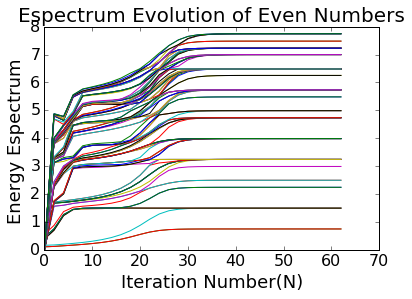
\includegraphics[scale=0.5]{IMAGES/even.png}}\subfloat[$N$ run only through odd values]{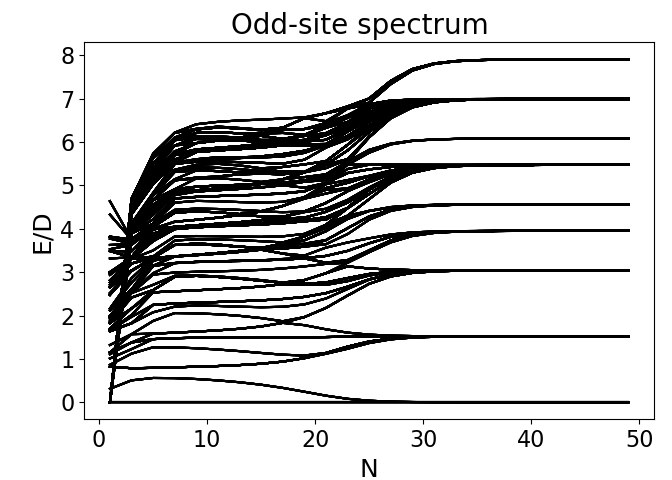
\includegraphics[scale=0.5]{IMAGES/odd.png}}\caption{\label{Fig-Dot-Spectrum} Evolution of the QD-spectrum vs number of
	iterations of the code for $U=0.5,\ e_{d}=-0.25,\ \Gamma=2.82\times10^{-2}.$ }
\end{figure}

The next step would be to diagonalize $H_{0}$ by blocks $H_{\mathcal{N},S}$ and then including the next place in the chain. The following Hamiltonians are generated in the same way from equation \ref{eq:NRG-Renormalization}. The symmetries of the new states can be obtained from the propagation rule \ref{eq:PropRuleQD}. When the number of states surpasses the 1000 states, the code will automatically cutoff the higher energy states. However it is important that a Block is not divided in this cutting, since it could break the preserved symmetry. 

Finally, the spectrum for $\Lambda = 2.5$ takes the 'spaghetti' form in \ref{Fig-Dot-Spectrum}. Before $N=30$ low-energy contributions generate significant changes in the energy levels.  The stable strum after the step $N=30$ shows that the code has converged at this stage. As we previously declared, it is not $\mathcal{T}$ but $\mathcal{T}^2$ the transformation that has fixed points, which explains why it was necessary to plot the even and the odd spectrum separately.

% The resulting eigenvectors will be characterized by both quantum numbers
% so that we can write them in the form $\vert N,S,i\rangle$ with $i$
% taking as many values as the degeneracy of its block. For higher values of $N$,

% We now proceed by induction supposing that for each $N$ the Hamiltonian $H_{N}$ is already diagonalized and the eigenvectors are organized in states with labels $\vert N,S,i\rangle.$ The next step will be to add the $4$-Hilbert space corresponding to $f_{N+1,\sigma}$ organized the eigenvectors according to the quantum numbers $\vert N',S',i\rangle$ and proceed to diagonalize by blocks the new Hamiltonian. Apart of it, the code must have a cutoff to the number of states. \\

At the end of the NRG code, we obtain a complete list of the spectrum $(E_{i, N})$ and the eigenstates $(\vert i , N \rangle)$ of the Hamiltonian at each step $N$ of the chain ( See \ref{Fig-Dot-Spectrum}). It is important to keep all of these states since each one of them represents different thermodynamic regimes of the system. While the site $N=1$ represents the physics of the system relevant at temperatures around $K_B D \Lambda^{-1}$, the site $N=30$ shows the low energy contributions at $T \sim K_B D \Lambda^{-30}$ where the ground state is strongly correlated. Furthermore, the states at low temperatures are entangled with the higher energy states. We need to take this into account to extract dynamical quantities of the system, which is the objective of the following section. 

\subsection{The Density Matrix Renormalization Group (DM-NRG) \label{subsec:DM-NRG}}
The NRG codes allows us to compute several thermodynamic quantities such as the entropy $S$, the free energy and the partition function $Z(\beta)$. In addition, we can compute the spin magnetization or dynamical quantities such  the density of states, the magnetic susceptibility and the conductivity. To perform this we can use the spectrum obtained in the NRG code to define the Boltzman distribution of the system. Then we apply the usual methods of statistical mechanics.  

% It is necessary to embed NRG with the faculty to compute these operators at each step $N$ of the code. {} 

In this thesis we will focus in computing the density of states at the impurity (QD). For this, let $\vert j\rangle$ and $\vert q \rangle$ label a base of eigenstates of the Hamiltonian $H$. Now recall the definition of the time-ordered green function \ref{eq:TempGreen}

\begin{align}
G_{d,d^{\dagger}}(t)&=\left\langle \mathbb{T}\left[d(t)d^{\dagger}(0)\right]\right\rangle \\ \label{eq:MeanGreen}
&=\theta(t)\left\langle \left[e^{\frac{i}{\hbar}Ht}de^{-\frac{i}{\hbar}Ht}d^{\dagger}\right]\right\rangle +\theta(-t)\left\langle \left[d^{\dagger}e^{\frac{i}{\hbar}Ht}de^{\frac{-i}{\hbar}Ht}\right]\right\rangle \\
&=\theta(t)\sum_{\vert j\rangle,\vert q\rangle}p_{j}\langle j\vert e^{\frac{i}{\hbar}Ht}d\vert q\rangle\langle q\vert e^{-\frac{i}{\hbar}Ht}d^{\dagger}\vert j\rangle+\theta(-t)\sum_{\vert j\rangle,\vert q\rangle}p_{q}\langle q\vert d^{\dagger}e^{\frac{i}{\hbar}Ht}\vert j\rangle\langle j\vert de^{-\frac{i}{\hbar}Ht}\vert q\rangle\\
&=\theta(t)\sum_{\vert j\rangle,\vert q\rangle}p_{j}e^{\frac{-i}{\hbar}t\left(E_{j}-E_{q}\right)}\left\Vert \langle j\vert d\vert q\rangle\right\Vert ^{2}+\theta(-t)\sum_{\vert j\rangle,\vert q\rangle}p_{q}e^{\frac{i}{\hbar}t\left(E_{j}-E_{q}\right)}\left\Vert \langle j\vert d\vert q\rangle\right\Vert ^{2}
\end{align}

\noindent Where $p_{j}:=\frac{e^{-\beta E_{j}}}{Z(\beta)}$ defines the Boltzmann probability of the eigenstate $\vert j\rangle$ according to Hamiltonian $H$. 

It is known that the Fourier transform of an expression of the form ${\displaystyle e^{-ax}\theta(x)}$ is $\frac{1}{\omega+is-a}$. Then the Green function in the frequency space is 
\begin{equation}
\Green{d,d^{\dagger}}=\frac{1}{Z(\beta)}\sum_{\vert j\rangle,\vert q\rangle}{\displaystyle \frac{e^{-\beta E_{j}}+e^{-\beta E_{q}}}{\omega+is-E_{j}+E_{q}}}\left\Vert \langle j\vert d\vert q\rangle\right\Vert ^{2}
. \label{eq:greenT}
\end{equation}

\noindent From the imaginary part of \ref{eq:greenT} we obtain a formula for the spectral density in terms of the eigenstates and energies of the Hamiltonian 
\begin{equation}
\rho_{d}=\frac{1}{Z(\beta)}\sum_{\vert j\rangle,\vert q\rangle}{\displaystyle \left(e^{-\beta E_{j}}+e^{-\beta E_{q}} \right) \delta\left(\omega-E_{j}+E_{q} \right) } \left\Vert \langle j\vert d\vert q\rangle \right\Vert^{2}. \label{eq:DOSeigenstates}
\end{equation}

\noindent This new expression for the DOS can be integrated to NRG code in different ways . A first method created by Costi \textit{et al.} consisted in computing \eqref{eq:DOSeigenstates} with the eigenstates of each shell Hamiltonian $H_N$  \cite{costi_transport_1994}. It is necessary to take into account that the operator $\langle j\vert d\vert q\rangle\right\Vert$ is constantly rotating after each diagonalization procedure generating different representation. Then, an important part of Costi's algorithm is to obtain these new representations of $\langle j\vert d\vert q\rangle\right\Vert_N$ recursively starting from an input representation $\langle j\vert d\vert q\rangle\right\Vert_{N=0}$.

Although Costi's method predicts accurately the DOS at low-energies, it fails to fit the high energy levels. The method that corrects this problem receives the name of Density Matrix Numerical Renormalization Group (DMNRG) \cite{hofstetter_generalized_2000}. The main idea of DMNRG is to include the entanglement corrections with the lower energy-states using the density matrix formalism. For this, Hofstetter defines the density matrix at the last shell Hamiltonian $N_{max}$ $\hat{\rho}$ as the thermal mixed state 

\begin{equation}
\hat{\rho}_{N_{max}} = \sum_{j}e^{-\beta E_{j}}\vert j          \rangle_N_{max} \langle j\vert, \label{eq:rho_n}
\end{equation}

\noindent where the subindex $N_{max}$ pinpoints that $\vert j \rangle_N_{max} \langle j\vert$ is an eigenstate of the last shell Hamiltonian $H_{N_max}$. 

With this new density matrix we could rewrite \ref{eq:MeanGreen} as 
\begin{equation}
G_{d,d^{\dagger}}^{N_{max}}(t)\left = \text{Tr}\left(\hat{\rho}_{N_{max}}\mathbb{T}\left[\left\{ d^{\dagger},d\right\} \right]\right). 
\end{equation}
\noindent From the Green function $G_{d,d^{\dagger}}^{N_{max}}(t)\left$ we can obtain the density of states associated to the temperature $T_{N_max}$. Nevertheless, these results are not relevant at higher temperatures. 

\begin{figure}
\centering
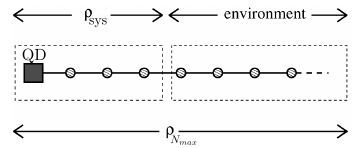
\includegraphics[scale=1]{IMAGES/DQD/DMRGchain.png}
\caption{\label{fig:OpenQuantum} Wilson's chain depicted as an open quantum system.  }
\end{figure}

To solve this problem we may think Wilson's chain as an open quantum system where the reservoir are the low-energy sites of the chain and the system contains the high energy site including the impurity/QD  as observed in \ref{fig:OpenQuantum}. Using this analogy it is possible we can readily obtain the density matrix $\rho_S$ by taking the partial trace over the reservoir

\begin{equation}
\rho_s = \text{Tr}_R[\rho_{N_{max}}].
\end{equation} 

The DM-NRG code applies recursively this idea to obtain the density matrix corresponding to each scale of temperature $T_N$. It starts from $\rho_{N_{max}}$ defined at \eqref{eq:rho_n} and obtains $\rho_{N_{max}-1} $ by taking the partial trace over the vector space corresponding to the last site of the chain
\begin{equation}
\rho_{N_{max}-1} = \text{Tr}_{N_{max}}[\rho_{N_{max}}].
\end{equation}
\noindent The other density matrices are computed by induction as 
\begin{equation}
\rho_{N-1} = \text{Tr}_{N}[\rho_{N}],
\end{equation}
and the density of states at each temperature regime can be computed at each stage from the green function 
\begin{equation}
G_{d,d^{\dagger}}^{N}(t)\left = \text{Tr}\left(\hat{\rho}_{N}\mathbb{T}\left[\left\{ d^{\dagger},d\right\} \right]\right). 
\end{equation}

The DM-NRG algorithm produces significantly better results  at high energies than Costi's initial idea. Indeed, DM-NRG is still one of the best methods to compute dynamic quantities of an impurity system. In the following subsection we will some details of how DM-NRG is integrated with the NRG code. 


% Then, we could rewrite equation  \ref{eq:MeanGreen} as 
% \begin{equation}
% G_{d,d^{\dagger}}(t)\left = \text{Tr}\left(\hat{\rho}_{N}\mathbb{T}\left[\left\{ d^{\dagger},d\right\} \right]\right). 
% \end{equation}
% But this result will only give us the result 


% But the density matrix $\hat{\rho}_{N}$ is different from \hat{\rho}_{N}$. In other 



% In this formalism the expression at

% However this last method neglected the strong correlation between the low and high energy states in the systems. 



% To compute  dynamical quantities  like the density of states we used the density matrix renormalization group approach . 



\subsection{Specifications of the NRG Code }

The NRG code used in this thesis was implemented by my thesis advisor Luis Gregorio Dias during his posdoc at the University of Ohio.  The general scheme  is shown in \ref{fig:Code}. It incorporates different stages in order to complete the procedure described in this classes. Here we give a brief description of each step:

\begin{figure}[t]
\centering
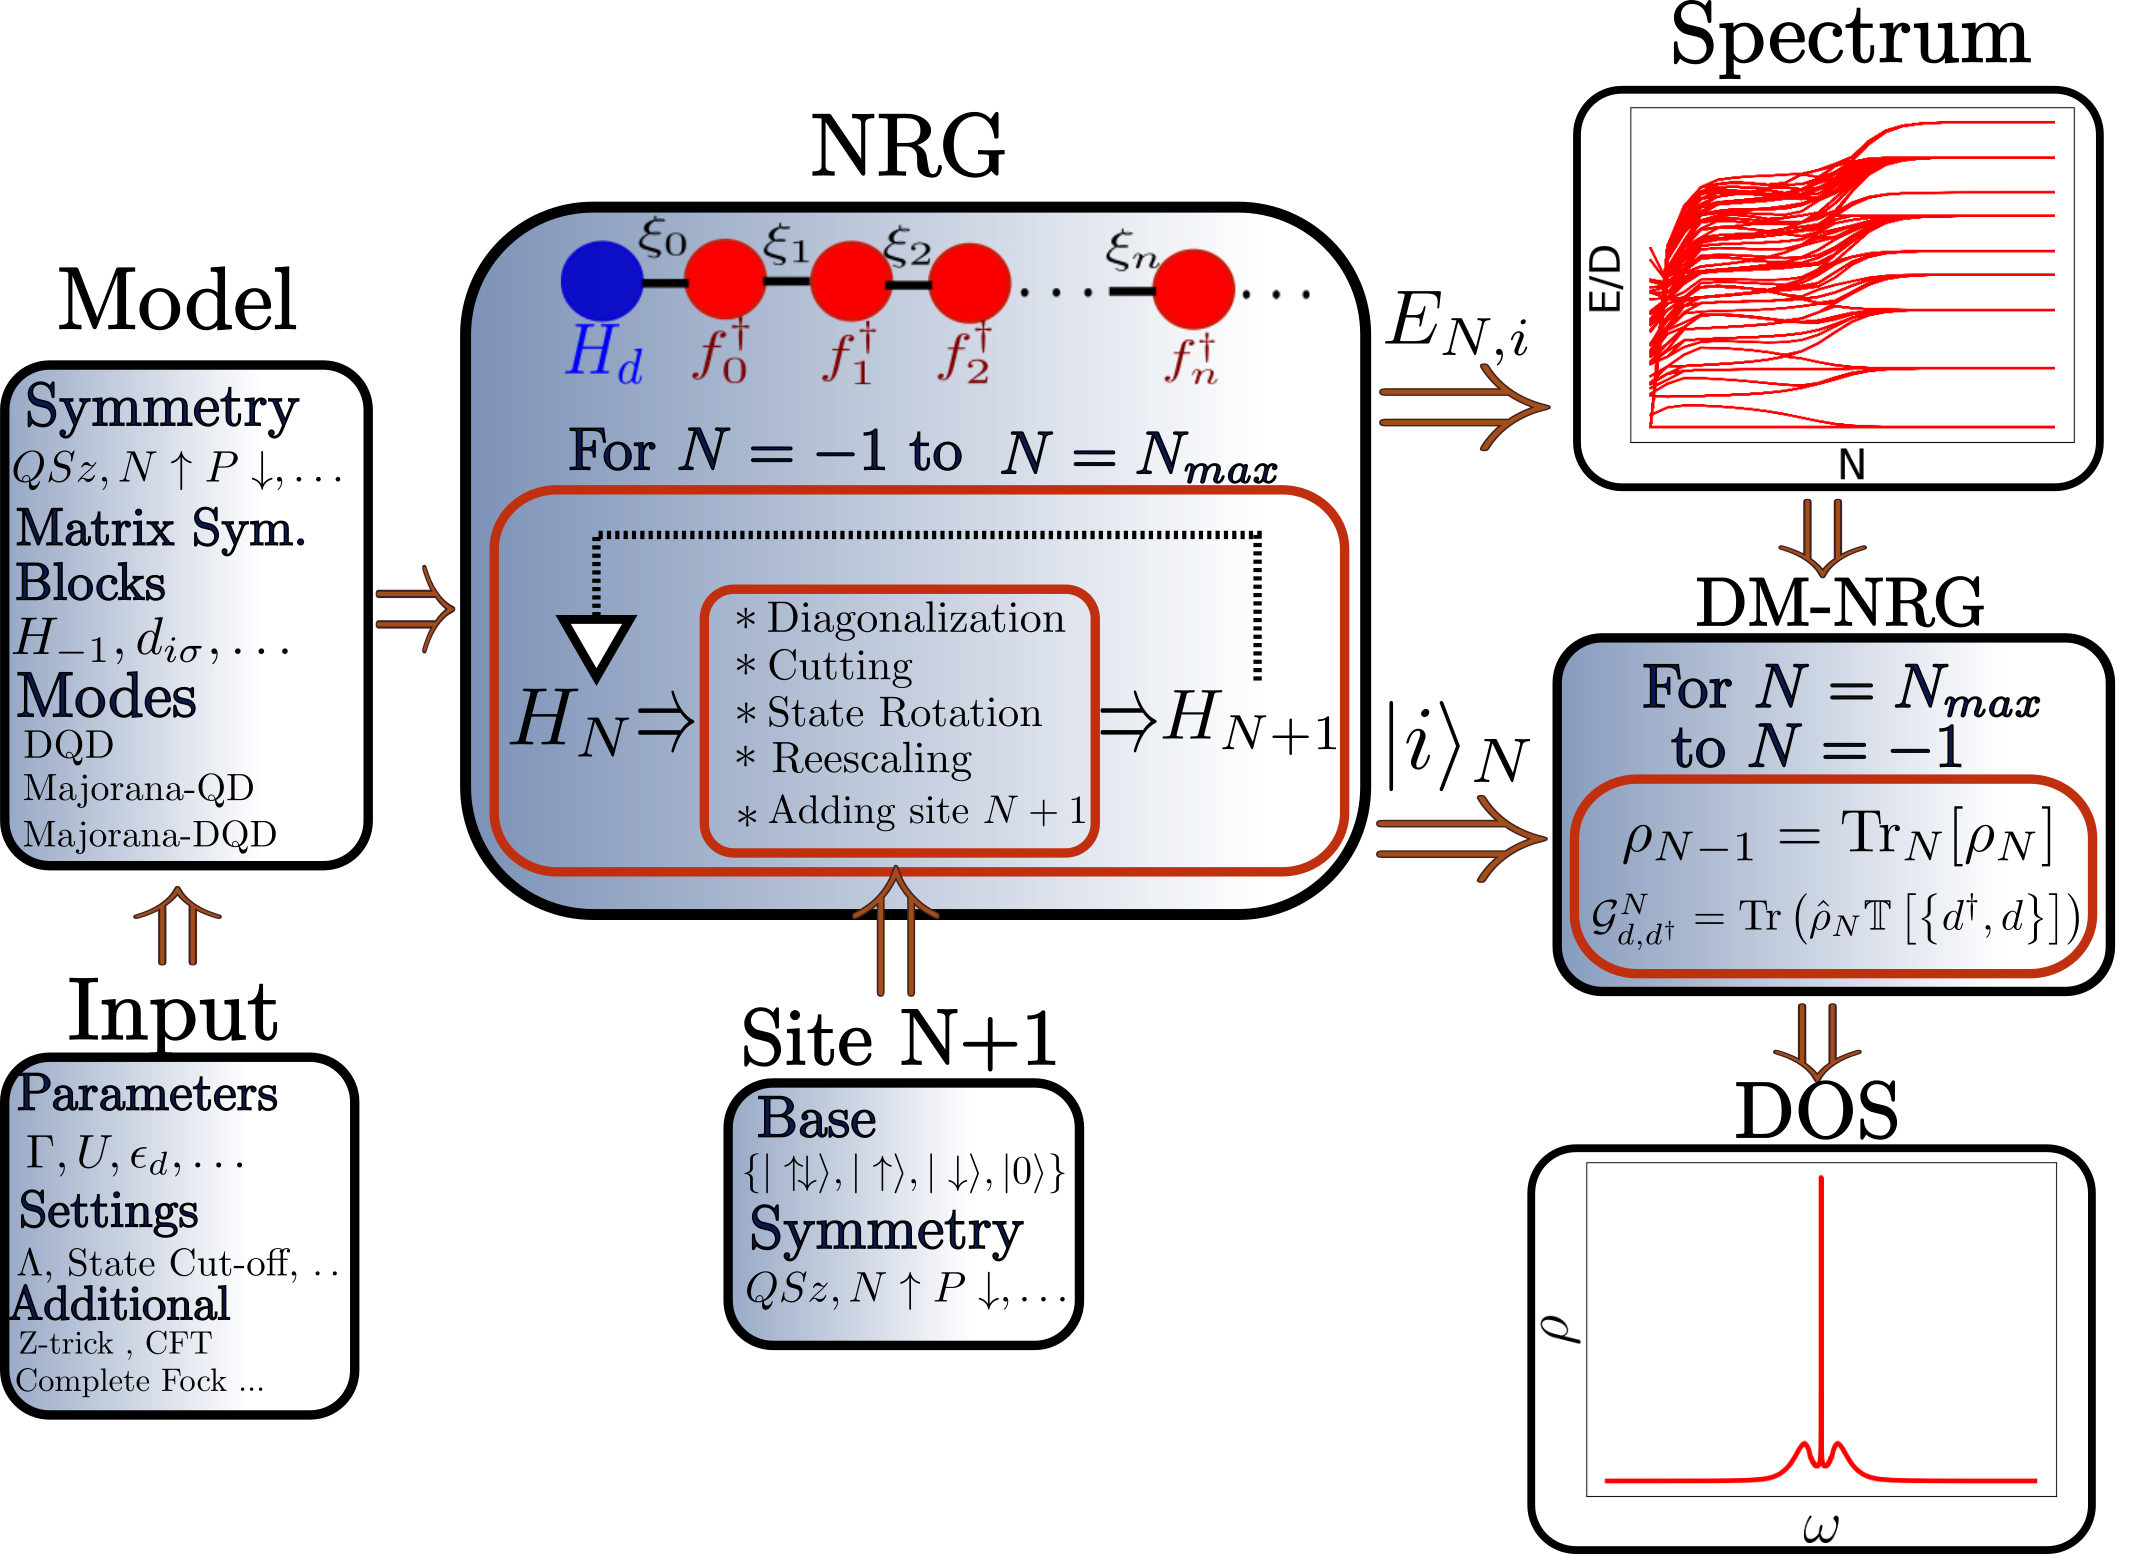
\includegraphics[scale=0.4]{IMAGES/NRG/NRGcode.png}
\caption{\label{fig:Code} Diagram of the NRG code}
\end{figure}

\begin{itemize}
\item \textbf{Model:} The model defines the type of impurity that we are going to study. It could be a single QD or more complex structures such as a DQD or a Majorana-QD system. My main contribution to this code was at this stage by designing the mode DQD-Majorana, which describes a DQD coupled to a Majorana zero mode. These models preserve different symmetries. In the single dot Hamiltonian presented in \ref{subsec:QD-Diag} we used the symmetry $\mathcal{N}S_z$, which is equivalent to charge-spin $QS_z$. However we will find that Majorana systems  require another  symmetry-type that we call as $N\up P\dw$. The model is defined by initial Hamiltonian $H_{-1}$ and the annihilation operators $d_{i\sigma}$ which must be submitted in the code written in the block symmetry representation described in \ref{subsec:Syms}.
\item \textbf{Input:} The input is a .dat file that attributes a numerical value to each parameter of the model. In addition, it allows to set different code specifications as the number of iterations $N_{max}$, the scaling parameter $\Lambda$ and the maximum number of states before the cut-off. It is also possible to include additional implementations to improve the results of the NRG code such as the Z-trick \cite{oliveira_generalized_1994} and the Complete Fock State. In this project, we only used the Z-trick, which significantly improves the spectral resolution at high energies.
\item \textbf{NRG-Main:} This part of the code mainly integrates the ideas of \ref{subsec:Logarithmic} and implements the iterative diagonalization described in \ref{subsec:IterativeDiag}. Each shell Hamiltonian $H_n$ is diagonalized. The high-energy eigenstates are cut-off if they exceed the limit. Then the states are rotated and the eigenvalues are rescaled to include the next step of the Wilson's chain. The symmetry block structure is preserved during the entire loop. NRG produces as out a detailed evolution of the spectrum which produces the spaghetti form. In addition, it can print the states and operators that are necessary to start other instances of the code like DM-NRG.
\item \textbf{Site $N+1$:} This is an small class that creates another site of the chain in the base $\left\{ \vert\uparrow\!\downarrow\rangle,\vert\uparrow\rangle,\vert\downarrow\rangle,\vert0\rangle\right\} $ . This base must be rewritten according to the symmetry quantum number to coupled it with the matrices at the NRG code. 
\item \textbf{DM-NRG}: As described in \ref{subsec:DM-NRG}, this code generates iteratively the density matrix associated to each energy scale. Then it computes the green function and the density of states. The DOS of the single $QD$ model is an example of its outputs. The plot shows the characteristic Kondo peak at the Fermi energy in the middle of the Coulomb peaks describing the energy states. 
\end{itemize}

 This NRG code was previously implemented in C++. It can be cloned from the Github link \url{https://git.io/fh9cM}.  To optimize the performance of NRG, the code uses the packages Boost, LAPACK and Gnu Scientific Library (GSL), which provide a rapid interface for numerical matrix diagonalization. 
 




  % language by the advisor of this thesis. In \ref{Fig-Dot-Spectrum} we observe the evolution of the spectrum of the Hamiltonian according to the number of iterations of the code. As we can appreciate, this evolution converges for even and odd number around $N=30$.  \\{}





\subsection{NRG results in a Double Quantum Dot Coupled to a Metallic Lead\label{sec: NRG-DQD}}

\begin{figure}[bt]
     \centering
    \subfloat[  \label{fig:NRG-1D}]{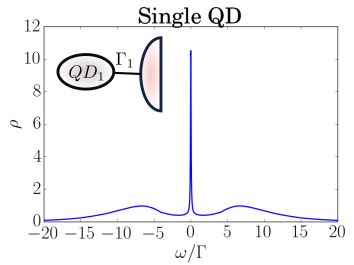
\includegraphics[scale=0.6]{IMAGES/DQD/NRG-QD.png}}
     \subfloat[$\Gamma_2 = \Gamma_1$ . Inset: Low energy DOS. \label{fig:NRGDQD-G2}]{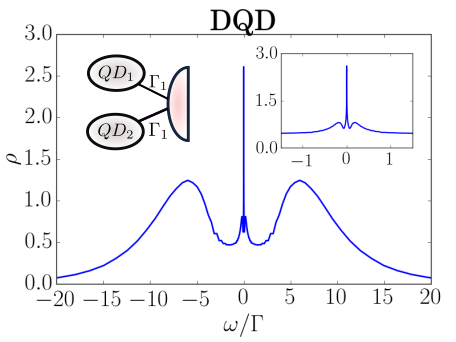
\includegraphics[scale=0.45]{IMAGES/DQD/NRG-DQD.png}} \\
    \subfloat[\label{fig:NRGDQD-tdots} $t_{dots}=0.689\Gamma$. Low energy DOS. ]{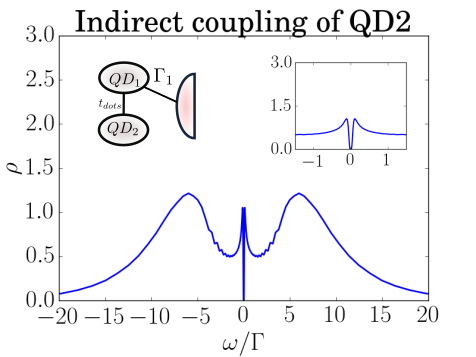
\includegraphics[scale=0.5]{IMAGES/DQD/NRG-IndirectDQD.png}}
    
     \caption{\label{fig:NRG-DQD} Density of states in QD1 predicted by NRG at each case.  The insets show the.  Note that figure a) is in a different scale due to a major central peak .. \protect\Source{ By the Author  }}
\end{figure}


We now intend to observe the results of this code applied to the model double quantum dot attached to a metallic lead.
The  Hamiltonian for this system is the Anderson model with the impurity given by the interacting version of Hamilonian \ref{eq:HDQD}

\begin{equation}
H_{DQD}=\sum_{i=1}^2\sum_\sigma \left( \epsilon_{i} + \frac{U_i}{2} \right) d_{i\sigma}^{\dagger}d_{i\sigma} + \left(\sum_{i\sigma} d_{i\sigma}^{\dagger}d_{i\sigma} -1 \right)^2 + \sum_\sigma t_{dots}d_{1\sigma}^{\dagger}d_{2\sigma}+t_{dots}^*d_{2\sigma}^{\dagger}d_{1\sigma}
\label{eq:interactingDQD}
\end{equation}

 The Hilbert space of this system has $16$-dimensions and the symmetries in this Hamiltonian are exactly the same than the ones in the single QD case $\mathcal{N}S$. Nevertheless, we decided to use the DQD-Majorana mode to simulate this system. By setting the Majorana couplings to $t_1=t_2= 0$ we can decouple the Majorana mode, hence obtaining the DQD model (See \ref{chap:Results}). The results we obtained are in agreement with previous previous works \cite{dias_da_silva_transmission_2008}, which was an important test to confirm the veracity of this new mode. 

For the entire thesis we will fix the value of the coulomb repulsion parameters to 
\begin{equation}
 U_1 = U_2 = 17.7305 \Gamma_1.
\end{equation}
\noindent We picked these parameters considerably higher than the broadening unit $\Gamma_1$ to guarantee the appearance of Kondo physics which is caused by these strong correlations. 

%Still need to correct this ... but for know.... PAPER!



 NRG-code  We used the same configurations from \ref{fig:GreenDQD}. 


%$$ -\ed{1,2} = \frac{U_{1,2}}{2}  = 8.62\Gamma_1$$

The single QD attached to a metallic lead is a particular case of the double quantum dot model, where the second dot is not attached $\Gamma_2 = t_{dots}=0$.  \ref{fig:NRG-DQD} shows the NRG results for this case. The three plots show the external Coulomb peaks at $e_1 = \frac{U}{2} \sim 8.62\Gamma_1$, which represent the DOS of the energy levels. In addition  Figure \ref{fig:NRG-1D} shows a central peak at the Fermi energy. \textbf{This is the Kondo Peak}. 

In Figure \ref{fig:NRGDQD-G2} we observe the DOS when the two QDs are symmetrically attached.  At low energies, the inset shows the appearance of two satellite peaks representing the Ruderman-Kittel-Kasuya-Yosida (RKKY) interaction. This is an anti-ferromagnetic coupling that appears in the interacting case due to the strong correlations between both dots. A detailed explanation of the appearance of these new states is included in section \ref{sec:DoublePeak}.  

The most interesting case is in Figure \ref{fig:NRGDQD-tdots}. As we already observed in the non-interacting case, the interference with the second dot completely destroys the Kondo peak. This effect is observed at low energies closed to $t_{dots}=0.689\Gamma$. The paper describing this result was a central part of one of my advisor's project. This result encouraged me to formulate the following question. What happens if we attached a Majorana mode to one of these dots?. Would it e destroyed by interference or it will survive to it. Answering this question is one of the mean objectives of chapter \ref{chap:Results}. 



%There is a problem with thes plots in xlabel.
